% Original lecture deck introducing hypothesis sets and PAC learning.
% Based primarily on Chapter 2 of:
% M. Mohri, A. Rostamizadeh, and A. Talwalkar,
% Foundations of Machine Learning, 2nd ed., MIT Press, 2018.
%
% No external images are required. All diagrams are drawn in TikZ.
% The source intentionally does not use \Huge or \huge.

\documentclass[aspectratio=169,10pt]{beamer}

\usepackage[T1]{fontenc}
\usepackage[utf8]{inputenc}
\usepackage{lmodern}
\usepackage{amsmath,amssymb,mathtools}
\usepackage{array,booktabs}
\usepackage{tikz}
\usetikzlibrary{arrows.meta,positioning,shapes.geometric,calc,fit,backgrounds}
\usepackage{hyperref}

% -----------------------------------------------------------------------------
% Visual style (compatible with the earlier COMP 5212 reconstructed decks)
% -----------------------------------------------------------------------------
\definecolor{slideorange}{HTML}{FF5500}
\definecolor{bulletgreen}{HTML}{A8C9A0}
\definecolor{bulletgray}{HTML}{D9E1E8}
\definecolor{deepblue}{HTML}{234A84}
\definecolor{softblue}{HTML}{EAF1FA}
\definecolor{softorange}{HTML}{FBEDE7}
\definecolor{softgreen}{HTML}{EDF5EB}
\definecolor{softgray}{HTML}{F2F3F5}
\definecolor{midgray}{HTML}{6A6A6A}
\definecolor{darkgreen}{HTML}{2F7A45}
\definecolor{darkred}{HTML}{A1261A}
\definecolor{pointblue}{HTML}{4E79A7}
\definecolor{pointred}{HTML}{D95F59}

\hypersetup{colorlinks=true,urlcolor=deepblue,linkcolor=deepblue}
\urlstyle{same}

\setbeamertemplate{navigation symbols}{}
\setbeamercolor{background canvas}{bg=white}
\setbeamercolor{normal text}{fg=black,bg=white}
\setbeamercolor{frametitle}{fg=slideorange,bg=white}
\setbeamercolor{page number in head/foot}{fg=black,bg=white}
\setbeamerfont{frametitle}{series=\bfseries,size*={25pt}{29pt}}
\setbeamerfont{page number in head/foot}{size=\scriptsize}
\setbeamersize{text margin left=0.90cm,text margin right=0.90cm}

\setbeamertemplate{frametitle}{%
  \vspace*{0.12cm}%
  \centering
  {\usebeamerfont{frametitle}\usebeamercolor[fg]{frametitle}\insertframetitle\par}%
  \vspace*{0.10cm}%
}

\setbeamertemplate{footline}{%
  \leavevmode
  \begin{beamercolorbox}[wd=\paperwidth,ht=0.42cm,dp=0.15cm,center]{page number in head/foot}
    \insertframenumber
  \end{beamercolorbox}%
}

\setbeamertemplate{itemize item}{%
  \raisebox{0.15ex}{\tikz\fill[bulletgreen] (0,0) circle (0.082cm);}%
}
\setbeamertemplate{itemize subitem}{%
  \raisebox{0.15ex}{\tikz\fill[bulletgray] (0,0) circle (0.064cm);}%
}

% -----------------------------------------------------------------------------
% Commands
% -----------------------------------------------------------------------------
\DeclareMathOperator*{\argmin}{arg\,min}
\newcommand{\X}{\mathcal{X}}
\newcommand{\Y}{\mathcal{Y}}
\newcommand{\D}{\mathcal{D}}
\newcommand{\C}{\mathcal{C}}
\newcommand{\Hc}{\mathcal{H}}
\newcommand{\Aalg}{\mathcal{A}}
\newcommand{\R}{R}
\newcommand{\Rhat}{\widehat{R}_S}
\newcommand{\ind}[1]{\mathbf{1}\!\left\{#1\right\}}
\newcommand{\eps}{\varepsilon}

\newcommand{\SectionSlide}[2]{%
  \begin{frame}
    \centering
    \vfill
    {\color{slideorange}\fontsize{29}{34}\selectfont\bfseries #1\par}
    \vspace{0.38cm}
    {\color{midgray}\fontsize{16}{21}\selectfont #2\par}
    \vfill
  \end{frame}
}

\newcommand{\SourceNote}[1]{%
  \vfill
  \begin{flushright}
    {\scriptsize\color{midgray}#1}
  \end{flushright}
}

\newcommand{\tightitems}{%
  \setlength{\itemsep}{0.14cm}%
  \setlength{\topsep}{0.08cm}%
  \setlength{\parsep}{0pt}%
}

\newcommand{\DefinitionBox}[1]{%
  \begin{beamercolorbox}[rounded=true,sep=0.22cm,wd=\linewidth]{block body}
    #1
  \end{beamercolorbox}%
}

\setbeamercolor{block body}{bg=softblue,fg=black}
\setbeamercolor{block title}{bg=deepblue,fg=white}
\setbeamercolor{alerted text}{fg=darkred}

\begin{document}

% -----------------------------------------------------------------------------
% 1. Title
% -----------------------------------------------------------------------------

\begin{frame}
	\begin{tikzpicture}[remember picture, overlay]
		\node[anchor=north west, inner sep=10pt] at (current page.north west)
		{
\includegraphics[width=6cm]{../source/logo.png}};
	\end{tikzpicture}
	
	\centering
	\vspace*{1.15cm}
	{\fontsize{28}{32}\selectfont COMP 5212\par}
	\vspace{0.35cm}
	{\fontsize{30}{33}\selectfont Machine Learning\par}
	\vspace{0.75cm}
	{\Large Instructor: Zihan Zhang\par}
	\vspace{0.35cm}
	{\large Lecture 2: Hypothesis Sets and PAC Learning\par}
	\vspace{0.2cm}
	
\end{frame}

% -----------------------------------------------------------------------------
% 2. Learning goals
% -----------------------------------------------------------------------------
\begin{frame}[t]{Learning Goals}
  \vspace{0.12cm}
  {\fontsize{14.5}{18}\selectfont
  By the end of this lecture, you should be able to:
  \begin{itemize}
    \setlength{\itemsep}{0.18cm}
    \item define a \textbf{hypothesis set} and explain its inductive bias;
    \item distinguish \textbf{empirical} from \textbf{generalization} error;
    \item state the basic \textbf{PAC-learning guarantee};
    \item derive the finite-class sample bound using a union bound;
    \item explain why infinite classes need a richer capacity measure.
  \end{itemize}}
\end{frame}

% -----------------------------------------------------------------------------
% 3. Motivation: an application case
% -----------------------------------------------------------------------------
\begin{frame}[t]{Application: Build a Spam Filter}
  \vspace{0.10cm}
  \centering
  {\fontsize{15}{18}\selectfont A new message arrives. Predict its label before it is seen.}
  \vspace{0.18cm}
  \begin{columns}[T,totalwidth=\textwidth]
    \begin{column}{0.45\textwidth}
      \begin{beamercolorbox}[rounded=true,sep=0.23cm,wd=\linewidth]{block body}
        \centering
        {\bfseries\large Incoming message}\par
        \vspace{0.12cm}
        \begin{beamercolorbox}[rounded=true,sep=0.13cm,wd=0.94\linewidth]{block body}
          \centering
          \normalsize
          \textbf{Subject:} FREE prize --- claim now!\\[0.08cm]
          \textbf{From:} news@shop.example
        \end{beamercolorbox}
        \vspace{0.14cm}
        \renewcommand{\arraystretch}{1.12}
        \begin{tabular}{@{}ll@{}}
          contains ``free'' & 1\\
          contains ``prize'' & 1\\
          known sender & 0
        \end{tabular}
      \end{beamercolorbox}
    \end{column}
    \begin{column}{0.51\textwidth}
      \begin{beamercolorbox}[rounded=true,sep=0.23cm,wd=\linewidth]{block body}
        {\bfseries\large Learning task}\par
        \vspace{0.10cm}
        \begin{itemize}
          \tightitems
          \item $x$: a feature vector describing the message;
          \item $y\in\{0,1\}$: not spam or spam;
          \item $S$: labeled messages collected in the past.
        \end{itemize}
        \vspace{0.05cm}
        \begin{beamercolorbox}[rounded=true,sep=0.13cm,wd=0.96\linewidth,center]{block body}
          \normalsize What kinds of rules should the learner be allowed to use?
        \end{beamercolorbox}
      \end{beamercolorbox}
    \end{column}
  \end{columns}
  \vspace{0.18cm}
  \begin{beamercolorbox}[rounded=true,sep=0.18cm,wd=0.94\linewidth,center]{block body}
    \centering
    Data will choose a rule, but we choose the \textbf{menu of allowable rules} first.
  \end{beamercolorbox}
  \note{[Sources] Application framing inspired by Avrim Blum, CMU 15-859(B), Lecture 1 (spam-filtering setup): https://www.cs.cmu.edu/~avrim/ML09a/lect0112.pdf}
\end{frame}

% -----------------------------------------------------------------------------
% 4. Motivation: make the menu explicit
% -----------------------------------------------------------------------------
\begin{frame}[t]{One Data Set, Three Rule Families}
  \vspace{0.05cm}
  \centering
  {\normalsize The training messages are fixed; the menu of allowed rules is a modeling choice.}
  \vspace{0.16cm}
  \begin{columns}[T,totalwidth=\textwidth]
    \begin{column}{0.32\textwidth}
      \begin{beamercolorbox}[rounded=true,sep=0.20cm,wd=\linewidth]{block body}
        \centering
        {\bfseries\textcolor{deepblue}{Keyword threshold}}\par
        \vspace{0.12cm}
        \[
          \Hc_1=\{\text{score thresholds}\}
        \]
        \small One score, one cut.\\[0.08cm]
        Simple and easy to estimate.
      \end{beamercolorbox}
    \end{column}
    \begin{column}{0.34\textwidth}
      \begin{beamercolorbox}[rounded=true,sep=0.20cm,wd=\linewidth]{block body}
        \centering
        {\bfseries\textcolor{darkgreen}{Conjunctions}}\par
        \vspace{0.12cm}
        \[
          \Hc_2=\{\text{word conjunctions}\}
        \]
        \small Example: ``free'' $\land$ ``prize''.\\[0.08cm]
        Encodes a sparse, interpretable rule.
      \end{beamercolorbox}
    \end{column}
    \begin{column}{0.32\textwidth}
      \begin{beamercolorbox}[rounded=true,sep=0.20cm,wd=\linewidth]{block body}
        \centering
        {\bfseries\textcolor{slideorange}{Memorization}}\par
        \vspace{0.12cm}
        \[
          \Hc_3=\{h:\X\to\{0,1\}\}
        \]
        \small Can fit every observed message.\\[0.08cm]
        Flexible, but prone to overfitting.
      \end{beamercolorbox}
    \end{column}
  \end{columns}
  \vspace{0.20cm}
  \begin{beamercolorbox}[rounded=true,sep=0.18cm,wd=0.94\linewidth,center]{block body}
    \centering
    The learner returns one $h_S\in\Hc$; the choice of $\Hc$ is the \textbf{inductive bias}.
  \end{beamercolorbox}
  \note{[Sources] Hypothesis-class framing follows Cornell CS4780 Lecture 1 (https://www.cs.cornell.edu/courses/cs4780/2018sp/lectures/lecturenote01_MLsetup.html) and MIT 6.036 Chapter 2 (https://openlearninglibrary.mit.edu/assets/courseware/v1/dc2ca4ef11bd7be3faec0efc56f46cca/asset-v1\%3AMITx\%2B6.036\%2B1T2019\%2Btype\%40asset\%2Bblock/notes_chapter_Linear_classifers.pdf).}
\end{frame}

% -----------------------------------------------------------------------------
% 5. Section
% -----------------------------------------------------------------------------
\SectionSlide{Hypothesis Sets}{What predictors may the learning algorithm choose?}

% -----------------------------------------------------------------------------
% 6. Learning pipeline
% -----------------------------------------------------------------------------
\begin{frame}[t]{From Data to a Predictor}
  \vspace{0.28cm}
  \begin{center}
  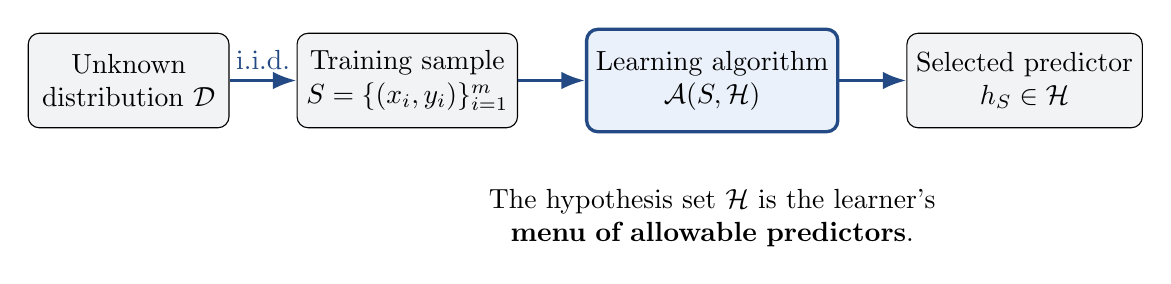
\begin{tikzpicture}[
      node distance=0.85cm and 0.85cm,
      box/.style={draw=black,rounded corners=4pt,minimum width=2.55cm,minimum height=1.20cm,align=center,fill=softgray},
      focus/.style={draw=deepblue,very thick,rounded corners=4pt,minimum width=2.75cm,minimum height=1.30cm,align=center,fill=softblue},
      arr/.style={-{Latex[length=3mm]},very thick,deepblue}
    ]
    \node[box] (dist) {Unknown\\distribution $\D$};
    \node[box,right=of dist] (sample) {Training sample\\$S=\{(x_i,y_i)\}_{i=1}^{m}$};
    \node[focus,right=of sample] (learner) {Learning algorithm\\$\Aalg(S,\Hc)$};
    \node[box,right=of learner] (hyp) {Selected predictor\\$h_S\in\Hc$};
    \draw[arr] (dist) -- node[above,midway]{i.i.d.} (sample);
    \draw[arr] (sample) -- (learner);
    \draw[arr] (learner) -- (hyp);
    \node[below=0.58cm of learner,align=center,text width=8.0cm] {
      \normalsize The hypothesis set $\Hc$ is the learner's \textbf{menu of allowable predictors}.
    };
  \end{tikzpicture}
  \end{center}
  \vspace{0.18cm}
  \begin{beamercolorbox}[rounded=true,sep=0.20cm,wd=0.94\linewidth,center]{block body}
    \centering
    Data select a predictor; the hypothesis set determines what can be selected.
  \end{beamercolorbox}
\end{frame}

% -----------------------------------------------------------------------------
% 5. Formal setup
% -----------------------------------------------------------------------------
\begin{frame}[t]{Formal Setup}
  \vspace{0.02cm}
  \begin{columns}[T,totalwidth=\textwidth]
    \begin{column}{0.42\textwidth}
      \begin{itemize}
        \setlength{\itemsep}{0.20cm}
        \item $\X$: instance space.
        \item $\Y=\{0,1\}$: label space.
        \item $c:\X\to\Y$: target concept.
        \item $\C$: possible target concepts.
        \item $\D$: unknown distribution on $\X$.
      \end{itemize}
    \end{column}
    \begin{column}{0.56\textwidth}
      \begin{beamercolorbox}[rounded=true,sep=0.20cm,wd=\linewidth]{block body}
        A labeled sample is
        \[
          S=\bigl((x_1,y_1),\ldots,(x_m,y_m)\bigr),
          \qquad y_i=c(x_i),
        \]
        with
        \[
          x_1,\ldots,x_m\overset{\mathrm{i.i.d.}}{\sim}\D.
        \]
        The learner sees $S$, but not $c$ or $\D$.
      \end{beamercolorbox}
      \vspace{0.18cm}
      Training and test inputs are assumed to follow the same $\D$.
    \end{column}
  \end{columns}
\end{frame}

% -----------------------------------------------------------------------------
% 6. Hypothesis set definition
% -----------------------------------------------------------------------------
\begin{frame}[t]{What Is a Hypothesis Set?}
  \vspace{0.24cm}
  \begin{beamercolorbox}[rounded=true,sep=0.28cm,wd=\linewidth]{block body}
    {\fontsize{16}{20}\selectfont
    A \textbf{hypothesis set} (or hypothesis class) is a collection
    \[
      \Hc\subseteq\{h:\X\to\Y\}
    \]
    of candidate prediction rules available to the learner.}
  \end{beamercolorbox}

  \vspace{0.34cm}
  {\normalsize
  \begin{itemize}
    \setlength{\itemsep}{0.27cm}
    \item The learning algorithm outputs $h_S\in\Hc$.
    \item $\Hc$ encodes an \textbf{inductive bias}: which explanations are considered plausible.
    \item Parameters index hypotheses; the entire parameterized family is the set $\Hc$.
  \end{itemize}}

  \vspace{0.14cm}
  \centering
  {\normalsize Example: $\Hc=\{x\mapsto \ind{w^Tx+b\ge 0}:w\in\mathbb{R}^d,b\in\mathbb{R}\}$.}
\end{frame}

% -----------------------------------------------------------------------------
% 7. Examples of H
% -----------------------------------------------------------------------------
\begin{frame}[t]{Examples of Hypothesis Sets}
  \vspace{-0.02cm}
  \begin{columns}[T,totalwidth=\textwidth]
    \begin{column}{0.32\textwidth}
      \centering
      {\bfseries Thresholds on a line}\par
      \vspace{0.12cm}
      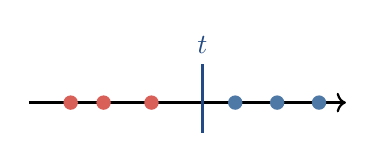
\begin{tikzpicture}[x=0.76cm,y=0.76cm]
        \draw[->,thick] (0,0)--(5.3,0);
        \draw[very thick,deepblue] (2.9,-0.5)--(2.9,0.65);
        \node[deepblue,above] at (2.9,0.65) {$t$};
        \foreach \x in {0.7,1.25,2.05}{\fill[pointred] (\x,0) circle (2.6pt);}
        \foreach \x in {3.45,4.15,4.85}{\fill[pointblue] (\x,0) circle (2.6pt);}
      \end{tikzpicture}
      \[
        h_t(x)=\ind{x\ge t}
      \]
    \end{column}
    \begin{column}{0.32\textwidth}
      \centering
      {\bfseries Intervals}\par
      \vspace{0.12cm}
      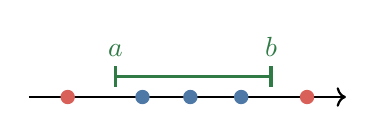
\begin{tikzpicture}[x=0.76cm,y=0.76cm]
        \draw[->,thick] (0,0)--(5.3,0);
        \draw[very thick,darkgreen] (1.45,0.34)--(4.05,0.34);
        \draw[very thick,darkgreen] (1.45,0.17)--(1.45,0.52);
        \draw[very thick,darkgreen] (4.05,0.17)--(4.05,0.52);
        \node[darkgreen,above] at (1.45,0.52) {$a$};
        \node[darkgreen,above] at (4.05,0.52) {$b$};
        \foreach \x in {0.65,4.65}{\fill[pointred] (\x,0) circle (2.6pt);}
        \foreach \x in {1.9,2.7,3.55}{\fill[pointblue] (\x,0) circle (2.6pt);}
      \end{tikzpicture}
      \[
        h_{a,b}(x)=\ind{a\le x\le b}
      \]
    \end{column}
    \begin{column}{0.34\textwidth}
      \centering
      {\bfseries Linear separators}\par
      \vspace{0.12cm}
      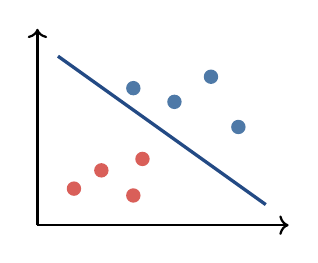
\begin{tikzpicture}[x=0.58cm,y=0.58cm]
        \draw[->,thick] (0,0)--(5.5,0);
        \draw[->,thick] (0,0)--(0,4.3);
        \draw[very thick,deepblue] (0.45,3.7)--(5.0,0.45);
        \foreach \p in {(0.8,0.8),(1.4,1.2),(2.1,0.65),(2.3,1.45)}{\fill[pointred] \p circle (2.6pt);}
        \foreach \p in {(2.1,3.0),(3.0,2.7),(3.8,3.25),(4.4,2.15)}{\fill[pointblue] \p circle (2.6pt);}
      \end{tikzpicture}
      \[
        h_{w,b}(x)=\ind{w^Tx+b\ge0}
      \]
    \end{column}
  \end{columns}
  \vspace{0.10cm}
  \begin{beamercolorbox}[rounded=true,sep=0.18cm,wd=0.94\linewidth,center]{block body}
    \centering
    A hypothesis set may be finite or infinite; its capacity, not just its parameter count, controls generalization.
  \end{beamercolorbox}
\end{frame}

% -----------------------------------------------------------------------------
% 8. Concept vs hypothesis set
% -----------------------------------------------------------------------------
\begin{frame}[t]{Concept Class vs. Hypothesis Set}
  \vspace{0.18cm}
  \begin{columns}[T,totalwidth=\textwidth]
    \begin{column}{0.49\textwidth}
      \begin{beamercolorbox}[rounded=true,sep=0.25cm,wd=\linewidth]{block body}
        {\normalsize
        \textbf{Concept class $\C$}\par
        \vspace{0.10cm}
        Describes possible data-generating target rules $c$.
        }
      \end{beamercolorbox}
      \vspace{0.25cm}
      \begin{beamercolorbox}[rounded=true,sep=0.25cm,wd=\linewidth]{block body}
        {\normalsize
        \textbf{Hypothesis set $\Hc$}\par
        \vspace{0.10cm}
        Describes predictors the algorithm is allowed to return.
        }
      \end{beamercolorbox}
    \end{column}
    \begin{column}{0.49\textwidth}
      \centering
      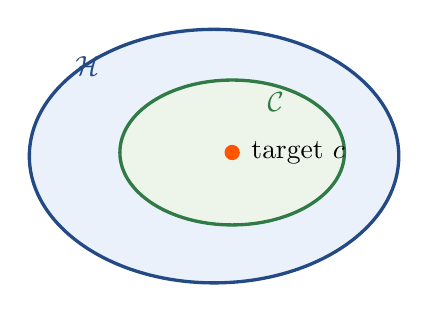
\begin{tikzpicture}[scale=0.92]
        \draw[very thick,deepblue,fill=softblue] (0,0) ellipse (2.55cm and 1.75cm);
        \draw[very thick,darkgreen,fill=softgreen] (0.25,0.05) ellipse (1.55cm and 1.00cm);
        \node[deepblue] at (-1.75,1.25) {$\Hc$};
        \node[darkgreen] at (0.85,0.75) {$\C$};
        \fill[slideorange] (0.25,0.05) circle (3.0pt);
        \node[right=0.12cm] at (0.25,0.05) {target $c$};
      \end{tikzpicture}
      \vspace{0.10cm}
      {\normalsize \textbf{Realizable case:} $c\in\Hc$.}
    \end{column}
  \end{columns}
  \vspace{0.34cm}
  {\normalsize
  If $c\notin\Hc$, the learner can only find the best approximation available inside $\Hc$; this is the \textbf{non-realizable} or \textbf{agnostic} setting.}
\end{frame}

% -----------------------------------------------------------------------------
% 9. Bias and capacity
% -----------------------------------------------------------------------------
\begin{frame}[t]{Hypothesis Sets Encode Inductive Bias}
  \vspace{0.08cm}
  \begin{center}
  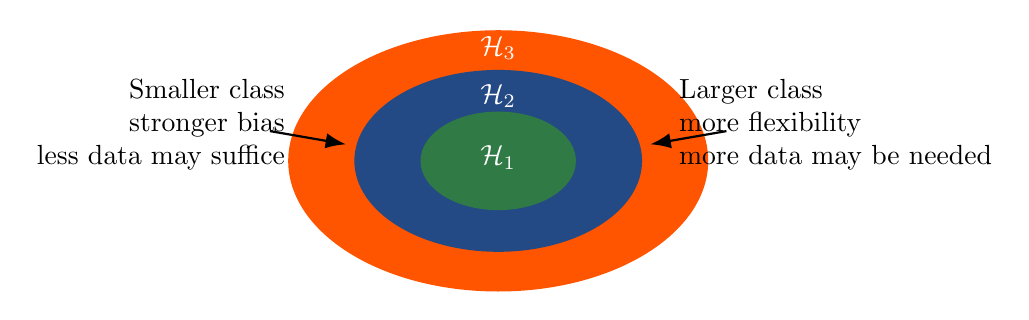
\begin{tikzpicture}[scale=0.84]
    \draw[very thick,fill=softorange,slideorange] (0,0) ellipse (3.15cm and 1.95cm);
    \draw[very thick,fill=softblue,deepblue] (0,0) ellipse (2.15cm and 1.35cm);
    \draw[very thick,fill=softgreen,darkgreen] (0,0) ellipse (1.15cm and 0.72cm);
    \node[white,font=\bfseries] at (0,0.05) {$\Hc_1$};
    \node[white,font=\bfseries] at (0,0.98) {$\Hc_2$};
    \node[white,font=\bfseries] at (0,1.70) {$\Hc_3$};
    \node[align=right] at (-5.1,0.55) {Smaller class\\stronger bias\\less data may suffice};
    \draw[-{Latex[length=2.6mm]},thick] (-3.45,0.45)--(-2.30,0.25);
    \node[align=left] at (5.1,0.55) {Larger class\\more flexibility\\more data may be needed};
    \draw[-{Latex[length=2.6mm]},thick] (3.45,0.45)--(2.30,0.25);
  \end{tikzpicture}
  \end{center}
  \vspace{0.05cm}
  \begin{columns}[T,totalwidth=\textwidth]
    \begin{column}{0.49\textwidth}
      \begin{beamercolorbox}[rounded=true,sep=0.18cm,wd=\linewidth,center]{block body}
        Too small $\Hc$: approximation error and underfitting.
      \end{beamercolorbox}
    \end{column}
    \begin{column}{0.49\textwidth}
      \begin{beamercolorbox}[rounded=true,sep=0.18cm,wd=\linewidth,center]{block body}
        Too rich $\Hc$: more data-fitting explanations and overfitting risk.
      \end{beamercolorbox}
    \end{column}
  \end{columns}
\end{frame}

% -----------------------------------------------------------------------------
% 10. Learning rules
% -----------------------------------------------------------------------------
\begin{frame}[t]{Learning Rules: ERM and Consistency}
  \vspace{0.06cm}
  A learning algorithm maps a sample to a hypothesis:
  \[
    \Aalg:S\longmapsto h_S\in\Hc.
  \]
  \vspace{-0.18cm}
  \begin{columns}[T,totalwidth=\textwidth]
    \begin{column}{0.49\textwidth}
      \begin{beamercolorbox}[rounded=true,sep=0.18cm,wd=\linewidth]{block body}
        \textbf{Empirical risk minimization (ERM)}
        \[
          h_S\in\argmin_{h\in\Hc}\widehat R_S(h).
        \]
        Choose the smallest training error.
      \end{beamercolorbox}
    \end{column}
    \begin{column}{0.49\textwidth}
      \begin{beamercolorbox}[rounded=true,sep=0.18cm,wd=\linewidth]{block body}
        \textbf{Consistent learning}
        \[
          \widehat R_S(h_S)=0.
        \]
        In a realizable problem, ERM can be consistent.
      \end{beamercolorbox}
    \end{column}
  \end{columns}
  \vspace{0.04cm}
  \begin{beamercolorbox}[rounded=true,sep=0.08cm,wd=0.92\linewidth,center]{block body}
    When does small training error imply small test error?
  \end{beamercolorbox}
\end{frame}

% -----------------------------------------------------------------------------
% 11. Risks
% -----------------------------------------------------------------------------
\begin{frame}[t]{Empirical Error vs. Generalization Error}
  \vspace{0.05cm}
  \begin{columns}[T,totalwidth=\textwidth]
    \begin{column}{0.49\textwidth}
      \begin{beamercolorbox}[rounded=true,sep=0.20cm,wd=\linewidth]{block body}
        \textbf{True error}
        \[
          R(h)=\Pr_{x\sim\D}[h(x)\ne c(x)].
        \]
        Performance on future examples.
      \end{beamercolorbox}
    \end{column}
    \begin{column}{0.49\textwidth}
      \begin{beamercolorbox}[rounded=true,sep=0.20cm,wd=\linewidth]{block body}
        \textbf{Empirical error}
        \[
          \widehat R_S(h)=\frac{1}{m}\sum_{i=1}^{m}\ind{h(x_i)\ne c(x_i)}.
        \]
        Performance on the training sample.
      \end{beamercolorbox}
    \end{column}
  \end{columns}
  \vspace{0.25cm}
  \begin{beamercolorbox}[rounded=true,sep=0.18cm,wd=0.94\linewidth,center]{block body}
    For a fixed $h$, $\widehat R_S(h)$ estimates $R(h)$. The subtlety is that the selected $h_S$ depends on $S$.
  \end{beamercolorbox}
\end{frame}

% -----------------------------------------------------------------------------
% 12. Version space
% -----------------------------------------------------------------------------
\begin{frame}[t]{Many Hypotheses Can Fit the Same Sample}
  \vspace{0.02cm}
  \begin{center}
  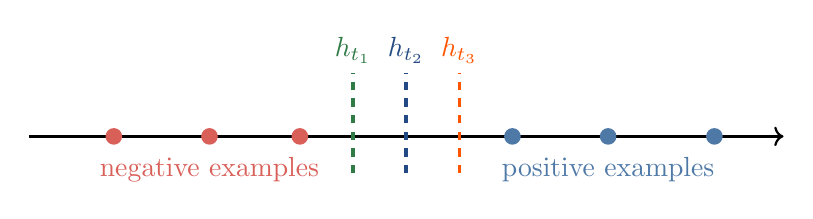
\begin{tikzpicture}[x=1.35cm,y=0.85cm]
    \draw[->,thick] (0,0)--(7.1,0);
    \foreach \x in {0.8,1.7,2.55}{\fill[pointred] (\x,0) circle (3pt);}
    \foreach \x in {4.55,5.45,6.45}{\fill[pointblue] (\x,0) circle (3pt);}
    \draw[dashed,very thick,darkgreen] (3.05,-0.55)--(3.05,0.95);
    \draw[dashed,very thick,deepblue] (3.55,-0.55)--(3.55,0.95);
    \draw[dashed,very thick,slideorange] (4.05,-0.55)--(4.05,0.95);
    \node[darkgreen,above] at (3.05,0.95) {$h_{t_1}$};
    \node[deepblue,above] at (3.55,0.95) {$h_{t_2}$};
    \node[slideorange,above] at (4.05,0.95) {$h_{t_3}$};
    \node[pointred,below] at (1.7,-0.16) {negative examples};
    \node[pointblue,below] at (5.45,-0.16) {positive examples};
  \end{tikzpicture}
  \end{center}
  \vspace{0.12cm}
  \begin{beamercolorbox}[rounded=true,sep=0.18cm,wd=0.90\linewidth,center]{block body}
    The \textbf{version space} is
    \[
      V_S=\{h\in\Hc:\widehat R_S(h)=0\}.
    \]
    PAC analysis asks whether every member of $V_S$ is likely to generalize.
  \end{beamercolorbox}
\end{frame}

% -----------------------------------------------------------------------------
% 13. Realizable case
% -----------------------------------------------------------------------------
\begin{frame}[t]{The Realizable Case}
  \vspace{0.24cm}
  {\fontsize{16}{20}\selectfont
  The basic PAC model begins with a favorable assumption:
  \[
    c\in\Hc.
  \]}
  \vspace{0.08cm}
  \begin{columns}[T,totalwidth=\textwidth]
    \begin{column}{0.48\textwidth}
      \begin{beamercolorbox}[rounded=true,sep=0.28cm,wd=\linewidth]{block body}
        {\normalsize \textbf{Consequence}\par
        A zero-training-error hypothesis exists for every sample.}
      \end{beamercolorbox}
    \end{column}
    \begin{column}{0.48\textwidth}
      \begin{beamercolorbox}[rounded=true,sep=0.28cm,wd=\linewidth]{block body}
        {\normalsize \textbf{Question}\par
        How large must $m$ be so that a consistent hypothesis has error at most $\eps$?}
      \end{beamercolorbox}
    \end{column}
  \end{columns}
  \vspace{0.40cm}
  \centering
  {\normalsize This leads to the Probably Approximately Correct framework.}
\end{frame}

% -----------------------------------------------------------------------------
% 14. Section PAC
% -----------------------------------------------------------------------------
\SectionSlide{PAC Learning}{A distribution-free, finite-sample notion of learnability}

% -----------------------------------------------------------------------------
% 15. PAC plain language
% -----------------------------------------------------------------------------
\begin{frame}[t]{PAC in Plain Language}
  \vspace{0.24cm}
  \begin{columns}[T,totalwidth=\textwidth]
    \begin{column}{0.32\textwidth}
      \begin{beamercolorbox}[rounded=true,sep=0.25cm,wd=\linewidth,center]{block body}
        \centering
        {\fontsize{18}{22}\selectfont\bfseries Probably}\par
        \vspace{0.18cm}
        {\normalsize With probability at least $1-\delta$ over the random training sample.}
      \end{beamercolorbox}
    \end{column}
    \begin{column}{0.32\textwidth}
      \begin{beamercolorbox}[rounded=true,sep=0.25cm,wd=\linewidth,center]{block body}
        \centering
        {\fontsize{18}{22}\selectfont\bfseries Approximately}\par
        \vspace{0.18cm}
        {\normalsize The returned predictor may not be perfect, but its error is at most $\eps$.}
      \end{beamercolorbox}
    \end{column}
    \begin{column}{0.32\textwidth}
      \begin{beamercolorbox}[rounded=true,sep=0.25cm,wd=\linewidth,center]{block body}
        \centering
        {\fontsize{18}{22}\selectfont\bfseries Correct}\par
        \vspace{0.18cm}
        {\normalsize Correctness is measured on new examples drawn from the unknown $\D$.}
      \end{beamercolorbox}
    \end{column}
  \end{columns}
  \vspace{0.45cm}
  \centering
  {\fontsize{17}{21}\selectfont PAC learning turns ``learns well'' into a statement involving $m$, $\eps$, and $\delta$.}
\end{frame}

% -----------------------------------------------------------------------------
% 16. Formal definition
% -----------------------------------------------------------------------------
\begin{frame}[t]{PAC-Learnability: Formal Definition}
  \vspace{0.04cm}
  \begin{beamercolorbox}[rounded=true,sep=0.22cm,wd=\linewidth]{block body}
    A concept class $\C$ is \textbf{PAC-learnable} if there exist a learner $\Aalg$ and a polynomial sample bound $m_{\C}$ such that, for every $c\in\C$, distribution $\D$, and $\eps,\delta\in(0,1)$, whenever $m\ge m_{\C}(\eps,\delta)$,
    \[
      \Pr_{S\sim\D^m}\!\left[R\bigl(\Aalg(S)\bigr)\le\eps\right]\ge 1-\delta.
    \]
  \end{beamercolorbox}
  \vspace{0.18cm}
  \begin{columns}[T,totalwidth=\textwidth]
    \begin{column}{0.32\textwidth}
      \centering\textbf{Universal}\par
      The guarantee holds for every target and every input distribution.
    \end{column}
    \begin{column}{0.32\textwidth}
      \centering\textbf{Probably}\par
      Probability is over the random training sample $S$.
    \end{column}
    \begin{column}{0.32\textwidth}
      \centering\textbf{Approximately correct}\par
      The returned error is at most $\eps$.
    \end{column}
  \end{columns}
  \SourceNote{Basic realizable PAC definition; Valiant (1984); Mohri et al. (2018), Chapter 2.}
\end{frame}

% -----------------------------------------------------------------------------
% 17. Assumptions
% -----------------------------------------------------------------------------
\begin{frame}[t]{What the Basic PAC Model Assumes}
  \vspace{0.18cm}
  \begin{columns}[T,totalwidth=\textwidth]
    \begin{column}{0.49\textwidth}
      \begin{beamercolorbox}[rounded=true,sep=0.25cm,wd=\linewidth]{block body}
        {\normalsize\bfseries Assumed}
        \begin{itemize}
          \tightitems
          \item examples are i.i.d.;
          \item training and test inputs share $\D$;
          \item the basic model is realizable: $c\in\Hc$;
          \item labels are binary in this presentation.
        \end{itemize}
      \end{beamercolorbox}
    \end{column}
    \begin{column}{0.49\textwidth}
      \begin{beamercolorbox}[rounded=true,sep=0.25cm,wd=\linewidth]{block body}
        {\normalsize\bfseries Not assumed}
        \begin{itemize}
          \tightitems
          \item a known parametric form for $\D$;
          \item Gaussian inputs or balanced classes;
          \item a particular learning algorithm;
          \item a specific geometry of $\X$.
        \end{itemize}
      \end{beamercolorbox}
    \end{column}
  \end{columns}
  \vspace{0.35cm}
  \centering
  {\normalsize PAC is \textbf{distribution-free}, but it does not cover arbitrary distribution shift.}
\end{frame}

% -----------------------------------------------------------------------------
% 18. Epsilon delta
% -----------------------------------------------------------------------------
\begin{frame}[t]{How to Read $\eps$ and $\delta$}
  \vspace{0.20cm}
  \begin{columns}[T,totalwidth=\textwidth]
    \begin{column}{0.48\textwidth}
      \begin{beamercolorbox}[rounded=true,sep=0.30cm,wd=\linewidth]{block body}
        \centering
        {\fontsize{18}{22}\selectfont\bfseries Accuracy $\eps$}\par
        \vspace{0.20cm}
        {\normalsize We want
        \[
          R(h_S)\le\eps.
        \]
        Smaller $\eps$ means a more accurate predictor and usually requires more data.}
      \end{beamercolorbox}
    \end{column}
    \begin{column}{0.48\textwidth}
      \begin{beamercolorbox}[rounded=true,sep=0.30cm,wd=\linewidth]{block body}
        \centering
        {\fontsize{18}{22}\selectfont\bfseries Failure probability $\delta$}\par
        \vspace{0.20cm}
        {\normalsize We want the guarantee to hold with probability
        \[
          1-\delta.
        \]
        Smaller $\delta$ means higher confidence and usually requires more data.}
      \end{beamercolorbox}
    \end{column}
  \end{columns}
  \vspace{0.40cm}
  \centering
  {\normalsize Example: $\eps=0.05$, $\delta=0.01$ means error at most $5\%$ with at least $99\%$ confidence.}
\end{frame}

% -----------------------------------------------------------------------------
% 19. Sample complexity
% -----------------------------------------------------------------------------
\begin{frame}[t]{Sample Complexity}
  \vspace{0.05cm}
  \begin{beamercolorbox}[rounded=true,sep=0.20cm,wd=\linewidth]{block body}
    The \textbf{sample complexity} $m_{\Hc}(\eps,\delta)$ is the number of labeled examples sufficient for a PAC guarantee over $\Hc$.
  \end{beamercolorbox}
  \vspace{0.18cm}
  It records how data requirements scale with:
  \begin{itemize}
    \setlength{\itemsep}{0.18cm}
    \item desired accuracy $1/\eps$;
    \item desired confidence $\ln(1/\delta)$;
    \item the complexity of $\Hc$;
    \item realizable versus agnostic assumptions.
  \end{itemize}
  \vspace{0.12cm}
  \begin{beamercolorbox}[rounded=true,sep=0.16cm,wd=0.94\linewidth,center]{block body}
    Efficient PAC learning additionally requires polynomial running time.
  \end{beamercolorbox}
\end{frame}

% -----------------------------------------------------------------------------
% 20. Finite H theorem
% -----------------------------------------------------------------------------
\begin{frame}[t]{Finite $\Hc$: Consistent Learning Bound}
  \vspace{0.04cm}
  \begin{columns}[T,totalwidth=\textwidth]
    \begin{column}{0.38\textwidth}
      \textbf{Assume:}
      \begin{itemize}
        \setlength{\itemsep}{0.17cm}
        \item $\Hc$ is finite;
        \item $c\in\Hc$;
        \item the learner returns $h_S$ with $\widehat R_S(h_S)=0$.
      \end{itemize}
    \end{column}
    \begin{column}{0.60\textwidth}
      \begin{beamercolorbox}[rounded=true,sep=0.20cm,wd=\linewidth]{block body}
        With probability at least $1-\delta$,
        \[
          R(h_S)\le \frac{\ln|\Hc|+\ln(1/\delta)}{m}.
        \]
      \end{beamercolorbox}
      \vspace{0.10cm}
      \begin{beamercolorbox}[rounded=true,sep=0.18cm,wd=\linewidth]{block body}
        Thus, to ensure $R(h_S)\le\eps$, it suffices that
        \[
          \boxed{m\ge \frac{\ln|\Hc|+\ln(1/\delta)}{\eps}}.
        \]
      \end{beamercolorbox}
    \end{column}
  \end{columns}
\end{frame}

% -----------------------------------------------------------------------------
% 21. Proof fixed bad h
% -----------------------------------------------------------------------------
\begin{frame}[t]{Proof Idea I: A Bad Hypothesis Is Unlikely to Look Perfect}
  \vspace{0.02cm}
  \begin{columns}[T,totalwidth=\textwidth]
    \begin{column}{0.51\textwidth}
      Fix $h$ with $R(h)>\eps$. Each example falls in the error region with probability greater than $\eps$.
      \vspace{0.10cm}
      \[
        \Pr\!\left[\widehat R_S(h)=0\right]
        \le (1-\eps)^m
        \le e^{-m\eps}.
      \]
      A bad hypothesis can look perfect only if all $m$ examples miss its error region.
    \end{column}
    \begin{column}{0.46\textwidth}
      \centering
      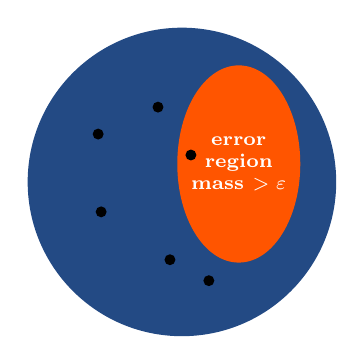
\begin{tikzpicture}[scale=0.76]
        \draw[very thick,fill=softblue,deepblue] (0,0) circle (2.55cm);
        \draw[very thick,fill=softorange,slideorange] (0.95,0.30) ellipse (1.00cm and 1.62cm);
        \node[white,align=center,font=\scriptsize\bfseries] at (0.95,0.30) {error\\region\\mass $>\eps$};
        \foreach \p in {(-1.4,0.8),(-1.35,-0.5),(-0.4,1.25),(-0.2,-1.3),(0.15,0.45),(0.45,-1.65)}
          {\fill[black] \p circle (2.6pt);}
      \end{tikzpicture}
    \end{column}
  \end{columns}
\end{frame}

% -----------------------------------------------------------------------------
% 22. Union bound
% -----------------------------------------------------------------------------
\begin{frame}[t]{Proof Idea II: Union Bound over All Bad Hypotheses}
  \vspace{0.02cm}
  Define
  \[
    \Hc_{\eps}=\{h\in\Hc:R(h)>\eps\}.
  \]
  The learner fails only if some bad hypothesis is consistent:
  \begin{align*}
    \Pr\!\left[\exists h\in\Hc_{\eps}:\widehat R_S(h)=0\right]
    &\le \sum_{h\in\Hc_{\eps}}\Pr\!\left[\widehat R_S(h)=0\right] \\
    &\le |\Hc|e^{-m\eps}.
  \end{align*}
  \vspace{-0.12cm}
  \begin{beamercolorbox}[rounded=true,sep=0.08cm,wd=0.88\linewidth,center]{block body}
    Set $|\Hc|e^{-m\eps}\le\delta$ and solve:
    \[
      m\ge\frac{\ln|\Hc|+\ln(1/\delta)}{\eps}.
    \]
  \end{beamercolorbox}
\end{frame}

% -----------------------------------------------------------------------------
% 23. Interpretation
% -----------------------------------------------------------------------------
\begin{frame}[t]{What the Finite-Class Bound Tells Us}
  \vspace{0.04cm}
  \renewcommand{\arraystretch}{1.28}
  \begin{center}
  \small
  \begin{tabular}{>{\bfseries}p{0.22\textwidth} p{0.65\textwidth}}
    \toprule
    Dependence & Interpretation \\
    \midrule
    $1/\eps$ & Halving the target error roughly doubles the required sample size. \\
    $\ln(1/\delta)$ & High confidence costs only logarithmically more data. \\
    $\ln|\Hc|$ & The number of candidates enters through its logarithm. \\
    consistency & The fast $1/m$ rate uses realizability and zero training error. \\
    \bottomrule
  \end{tabular}
  \end{center}
  \vspace{0.16cm}
  \begin{beamercolorbox}[rounded=true,sep=0.16cm,wd=0.94\linewidth,center]{block body}
    $\log_2|\Hc|$ is the number of bits needed to identify a hypothesis: a formal version of \textbf{Occam's razor}.
  \end{beamercolorbox}
\end{frame}

% -----------------------------------------------------------------------------
% 24. Numerical example
% -----------------------------------------------------------------------------
\begin{frame}[t]{Numerical Example: Discretized Thresholds}
  \vspace{0.05cm}
  Suppose $|\Hc|=1001$ candidate thresholds and we want $\eps=0.05$, $\delta=0.05$.
  \vspace{0.12cm}
  \begin{beamercolorbox}[rounded=true,sep=0.20cm,wd=0.86\linewidth,center]{block body}
    \[
      m\ge
      \frac{\ln(1001)+\ln(20)}{0.05}
      \approx 198.1.
    \]
  \end{beamercolorbox}
  \vspace{0.20cm}
  \centering
  {\fontsize{18}{22}\selectfont\bfseries Therefore $m=199$ examples suffice under the theorem's assumptions.}
  \vspace{0.10cm}
  \begin{beamercolorbox}[rounded=true,sep=0.10cm,wd=0.88\linewidth,center]{block body}
    This is a worst-case guarantee, not a prediction of the exact data needed in a particular dataset.
  \end{beamercolorbox}
\end{frame}

% -----------------------------------------------------------------------------
% 25. Boolean conjunctions
% -----------------------------------------------------------------------------
\begin{frame}[t]{Example: Conjunctions of Boolean Literals}
  \vspace{0.12cm}
  {\normalsize Let $x\in\{0,1\}^n$. A conjunction can include each variable positively, negatively, or not at all:}
  \[
    h(x)=x_1\wedge \neg x_4\wedge x_7.
  \]
  \vspace{-0.05cm}
  {\normalsize Thus there are at most}
  \[
    |\Hc|=3^n
  \]
  {\normalsize conjunctions, and consistent PAC learning needs}
  \[
    m\ge \frac{n\ln 3+\ln(1/\delta)}{\eps}.
  \]
  \vspace{0.12cm}
  \begin{beamercolorbox}[rounded=true,sep=0.22cm,wd=0.90\linewidth,center]{block body}
    \centering
    {\normalsize For $n=20$, $\eps=0.10$, and $\delta=0.05$, the bound gives $m\ge 250$.}
  \end{beamercolorbox}
\end{frame}

% -----------------------------------------------------------------------------
% 26. Section beyond realizability
% -----------------------------------------------------------------------------
\SectionSlide{Beyond the Realizable Case}{Noisy labels, model mismatch, and uniform convergence}

% -----------------------------------------------------------------------------
% 27. Non-realizable
% -----------------------------------------------------------------------------
\begin{frame}[t]{When No Hypothesis Is Perfectly Consistent}
  \vspace{0.18cm}
  \begin{columns}[T,totalwidth=\textwidth]
    \begin{column}{0.52\textwidth}
      {\normalsize Real data may violate $c\in\Hc$:}
      \begin{itemize}
        \setlength{\itemsep}{0.28cm}
        \item labels can be noisy or stochastic;
        \item the chosen model family may be misspecified;
        \item several labels may be plausible for the same input.
      \end{itemize}
    \end{column}
    \begin{column}{0.45\textwidth}
      \begin{beamercolorbox}[rounded=true,sep=0.28cm,wd=\linewidth]{block body}
        {\normalsize In the \textbf{agnostic setting}, compare the learner to the best hypothesis in $\Hc$:
        \[
          h^*\in\argmin_{h\in\Hc}R(h).
        \]
        The goal is small \textbf{excess risk}
        \[
          R(h_S)-R(h^*).
        \]}
      \end{beamercolorbox}
    \end{column}
  \end{columns}
  \vspace{0.30cm}
  \centering
  {\normalsize We now need training and true errors to be close \emph{uniformly} over $\Hc$.}
\end{frame}

% -----------------------------------------------------------------------------
% 28. Hoeffding fixed h
% -----------------------------------------------------------------------------
\begin{frame}[t]{Hoeffding's Inequality for a Fixed Hypothesis}
  \vspace{0.14cm}
  {\normalsize For a fixed $h$, the $0$--$1$ losses are independent Bernoulli random variables. Hoeffding's inequality gives}
  \begin{beamercolorbox}[rounded=true,sep=0.25cm,wd=0.84\linewidth,center]{block body}
    \centering
    {\fontsize{16}{20}\selectfont
    \[
      \Pr\!\left[\left|R(h)-\widehat R_S(h)\right|>\gamma\right]
      \le 2e^{-2m\gamma^2}.
    \]}
  \end{beamercolorbox}
  \vspace{0.25cm}
  \begin{alertblock}{Why this is not yet enough}
    The output $h_S$ is \textbf{not fixed}; it depends on the same sample $S$ used to compute $\widehat R_S(h_S)$.
  \end{alertblock}
  \vspace{0.12cm}
  \centering
  {\normalsize We need one event on which the bound holds simultaneously for every $h\in\Hc$.}
\end{frame}

% -----------------------------------------------------------------------------
% 29. Uniform convergence
% -----------------------------------------------------------------------------
\begin{frame}[t]{Uniform Convergence for Finite $\Hc$}
  \vspace{0.04cm}
  Apply Hoeffding to every $h\in\Hc$ and use a union bound.
  \vspace{0.10cm}
  \begin{beamercolorbox}[rounded=true,sep=0.20cm,wd=0.92\linewidth,center]{block body}
    With probability at least $1-\delta$,
    \[
      \forall h\in\Hc,\qquad
      \left|R(h)-\widehat R_S(h)\right|
      \le
      \sqrt{\frac{\ln\!\left(2|\Hc|/\delta\right)}{2m}}.
    \]
  \end{beamercolorbox}
  \vspace{0.18cm}
  \centering
  Uniform convergence lets us compare all hypotheses using the same training sample.
\end{frame}

% -----------------------------------------------------------------------------
% 30. ERM guarantee
% -----------------------------------------------------------------------------
\begin{frame}[t]{ERM Guarantee in the Agnostic Setting}
  \vspace{0.02cm}
  Let $\widehat h$ minimize empirical risk, let $h^*$ minimize true risk over $\Hc$, and define
  \[
    \gamma_m=\sqrt{\frac{\ln(2|\Hc|/\delta)}{2m}}.
  \]
  On the uniform-convergence event,
  \[
    R(\widehat h)
    \le \widehat R_S(\widehat h)+\gamma_m
    \le \widehat R_S(h^*)+\gamma_m
    \le R(h^*)+2\gamma_m.
  \]
  \vspace{0.08cm}
  \begin{beamercolorbox}[rounded=true,sep=0.15cm,wd=0.90\linewidth,center]{block body}
    \[
      R(\widehat h)\le \min_{h\in\Hc}R(h)
      +2\sqrt{\frac{\ln(2|\Hc|/\delta)}{2m}}.
    \]
  \end{beamercolorbox}
\end{frame}

% -----------------------------------------------------------------------------
% 31. Approximation-estimation
% -----------------------------------------------------------------------------
\begin{frame}[t]{Approximation and Estimation}
  \vspace{0.16cm}
  \begin{center}
  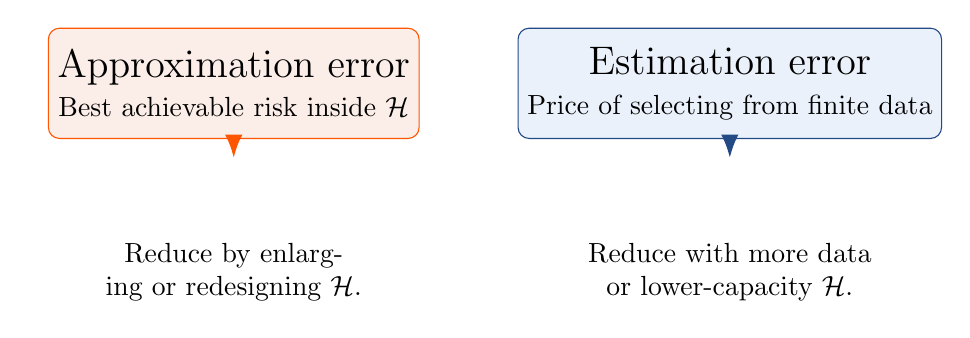
\begin{tikzpicture}[
      box/.style={draw,rounded corners=4pt,minimum width=4.7cm,minimum height=1.4cm,align=center},
      arr/.style={-{Latex[length=3mm]},very thick}
    ]
    \node[box,fill=softorange,draw=slideorange] (approx) at (-3.15,0) {\Large Approximation error\\[0.08cm]\normalsize Best achievable risk inside $\Hc$};
    \node[box,fill=softblue,draw=deepblue] (estim) at (3.15,0) {\Large Estimation error\\[0.08cm]\normalsize Price of selecting from finite data};
    \node[below=1.2cm of approx,align=center,text width=5.0cm] {Reduce by enlarging or redesigning $\Hc$.};
    \node[below=1.2cm of estim,align=center,text width=5.0cm] {Reduce with more data or lower-capacity $\Hc$.};
    \draw[arr,slideorange] (approx.south)--(-3.15,-0.95);
    \draw[arr,deepblue] (estim.south)--(3.15,-0.95);
  \end{tikzpicture}
  \end{center}
  \vspace{0.20cm}
  \begin{beamercolorbox}[rounded=true,sep=0.22cm,wd=0.92\linewidth,center]{block body}
    \centering
    {\normalsize Model selection balances the two: a richer hypothesis set improves fit but increases the amount of evidence needed for reliable selection.}
  \end{beamercolorbox}
\end{frame}

% -----------------------------------------------------------------------------
% 32. Infinite H
% -----------------------------------------------------------------------------
\begin{frame}[t]{What About Infinite Hypothesis Sets?}
  \vspace{0.04cm}
  Many useful classes are infinite:
  \begin{itemize}
    \setlength{\itemsep}{0.16cm}
    \item real-valued thresholds;
    \item intervals with real endpoints;
    \item linear separators in $\mathbb{R}^d$.
  \end{itemize}
  \vspace{0.08cm}
  \begin{alertblock}{Problem}
    The finite-class term $\ln|\Hc|$ is no longer useful.
  \end{alertblock}
  \vspace{0.10cm}
  \begin{beamercolorbox}[rounded=true,sep=0.18cm,wd=0.92\linewidth,center]{block body}
    Measure how many distinct labelings $\Hc$ can realize on finite samples. This leads to \textbf{growth functions}, \textbf{VC dimension}, and \textbf{Rademacher complexity}.
  \end{beamercolorbox}
\end{frame}

% -----------------------------------------------------------------------------
% 33. Takeaways
% -----------------------------------------------------------------------------
\begin{frame}[t]{Key Takeaways}
  \vspace{0.10cm}
  {\fontsize{14}{17.5}\selectfont
  \begin{itemize}
    \setlength{\itemsep}{0.28cm}
    \item $\Hc$ is the learner's allowable predictor family and its inductive bias.
    \item PAC means $R(h_S)\le\eps$ with probability at least $1-\delta$.
    \item Finite, realizable classes need
      $m=O\!\bigl((\ln|\Hc|+\ln(1/\delta))/\eps\bigr)$ examples.
    \item In the agnostic case, ERM excess risk is
      $O\!\bigl(\sqrt{(\ln|\Hc|+\ln(1/\delta))/m}\bigr)$.
    \item Infinite classes require capacity measures beyond cardinality, such as VC dimension or Rademacher complexity.
  \end{itemize}}
\end{frame}

% -----------------------------------------------------------------------------
% 34. Check your understanding
% -----------------------------------------------------------------------------
\begin{frame}[t]{Check Your Understanding}
  \vspace{0.06cm}
  {\fontsize{14}{17.5}\selectfont
  \begin{enumerate}
    \setlength{\itemsep}{0.25cm}
    \item If $|\Hc|$ doubles, how much does the finite realizable sample bound increase?
    \item Why can a fixed-$h$ Hoeffding bound not be applied directly to the ERM output $h_S$?
    \item Give an example with $c\notin\Hc$. What is the correct comparison target?
    \item Which is more expensive in the consistent bound: dividing $\eps$ by $10$, or dividing $\delta$ by $10$?
  \end{enumerate}}
  \vfill
  \centering
  {\small\color{midgray}Next: VC dimension and guarantees for infinite hypothesis sets.}
\end{frame}

% -----------------------------------------------------------------------------
% 35. References
% -----------------------------------------------------------------------------
\begin{frame}[t]{References and Further Reading}
  \vspace{0.05cm}
  \small
  \begin{thebibliography}{9}
    \setlength{\itemsep}{0.22cm}
    \bibitem{mohri2018}
    Mehryar Mohri, Afshin Rostamizadeh, and Ameet Talwalkar.
    \newblock \emph{Foundations of Machine Learning}, 2nd edition.
    \newblock MIT Press, 2018. Chapter 2: The PAC Learning Framework.

    \bibitem{valiant1984}
    Leslie G. Valiant.
    \newblock A Theory of the Learnable.
    \newblock \emph{Communications of the ACM}, 27(11):1134--1142, 1984.

    \bibitem{hoeffding1963}
    Wassily Hoeffding.
    \newblock Probability Inequalities for Sums of Bounded Random Variables.
    \newblock \emph{Journal of the American Statistical Association}, 58(301):13--30, 1963.
  \end{thebibliography}
  \vspace{0.06cm}
  \centering
  {\scriptsize\color{midgray}Original instructional summary; definitions and finite-class bounds follow Chapter 2 of Mohri et al.}
\end{frame}

\end{document}
\end{document}
